% \setchapterpreamble[u]{\margintoc}
\chapter{Introduction}
\labch{intro}

Type theory is set at the interface between programming and formal logic,
feeding off and nourishing both worlds. Proof assistants can be built on it,
making them full-fledged programming languages as well, with the added benifit
of producing certified programs.

My main interest lies in the study of type theory while relying on the tools it
provides: I study type theory \emph{within} type theory.
As such I focused on the formalisation of type theory in the \Coq proof
assistant~\sidecite[-0.7cm]{coq} and particularly on two points:
\marginnote[0.7cm]{
  Reflection is defined in \arefsubsec{ett-def}, and weak equality in
  \arefsubsec{wtt}, both in \refch{flavours}.
}
\begin{itemize}
  \item How can we effectively turn a proof using a very strong notion of
  equality called \emph{reflection}, into a proof relying on a very weak notion
  of equality?
  \item How can we improve the trust in our system, in my case \Coq, using this
  system itself as a framework to study it?
\end{itemize}

\paradot{Contributions}
My contributions will mainly be found in \arefpart{elim-reflection} and
\arefpart{coq-in-coq} corresponding to the following published
articles~\sidecite{winterhalter:hal-01849166,sozeau2019coq,sozeau:hal-02167423}.
While the chapters before these two parts are mainly introductory and
corresponding to a rough state-of-the-art, they actually contain other
contributions, namely work I did with Andrej Bauer on the cardinal model
in \nrefch{models} that we did not publish, and work I did with Andrej Bauer
and Philipp Haselwarter on formalising type theory called
\ftt~\sidecite{formaltypetheory} and that I present briefly in
\nrefch{formalisation}.
\todo{Make some statements precise for the reader in a hurry? Or should I have
an abstract instead?}

\section{Proof assistants}
\todo{Very WIP}

One of my goals is improving and understanding better proof assistants, but what
is a proof assistant?
I think we can see them as chatbots---that is, those programs that you can
converse with---that are there to help you assert and prove theorems.
They are not particularly smart and will not get the job done for you, but they
are very annoying because they do not always understand what you say and you
have to be very precise or they will point out your mistakes.

\begin{center}
  
\includegraphics[width=0.6\textwidth]{coq-chatbot.pdf}
\end{center}

Here, I represent the user on the left, conversing with the proof assistant, on
the right, that I picture as a laptop with a rooster inside.

Let us now see in detail how such a conversation can go.

\begin{center}
  
\includegraphics[width=0.8\textwidth]{modern-art.pdf}
\end{center}

This piece of modern art will be the setting for the exchange between the user
and the proof assistant, and we will assume they both agree on it.
We have cats in boxes (although one of the cats is rather a lion), of different
colours, and subject to different gravitation forces.

At the beginning, the user makes their purpose know to the proof assistant,
saying for which theorem they require their assistance.

\begin{center}
  
\includegraphics[width=0.8\textwidth]{iwanterror.pdf}
\end{center}

The sentence above doesn't sound like a statement we can prove, and the proof
assistant will rightfully complain.

\begin{center}
  
\includegraphics[width=0.8\textwidth]{error-incomplete.pdf}
\end{center}

Indeed, we were to fast and forgot half of what we wanted to say. Next we give
it a complete sentence.

\begin{center}
  
\includegraphics[width=0.8\textwidth]{iwant-is.pdf}
\end{center}

This time, the statement is slightly incorrect, or not precise enough for our
good assistant.

\begin{center}
  
\includegraphics[width=0.8\textwidth]{error-box-feline.pdf}
\end{center}

We have to revise our wanted theorem, and realise that we do not want to prove
that all boxes are feline, although a human might understand what we mean by
that, but that all of the boxes contain, each, a feline.

\begin{center}
  
\includegraphics[width=0.8\textwidth]{box-contains-feline.pdf}
  
\includegraphics[width=0.8\textwidth]{how-to-prove.pdf}
\end{center}

The proof assistant has now understood what we meant. The interactive part of
the prove now begins. We want to prove a property on the boxes, as there are
four to consider, we can tell the proof assistant that we intend to look at each
case, one by one.

\begin{center}
  
\includegraphics[width=0.8\textwidth]{convo7.pdf}
  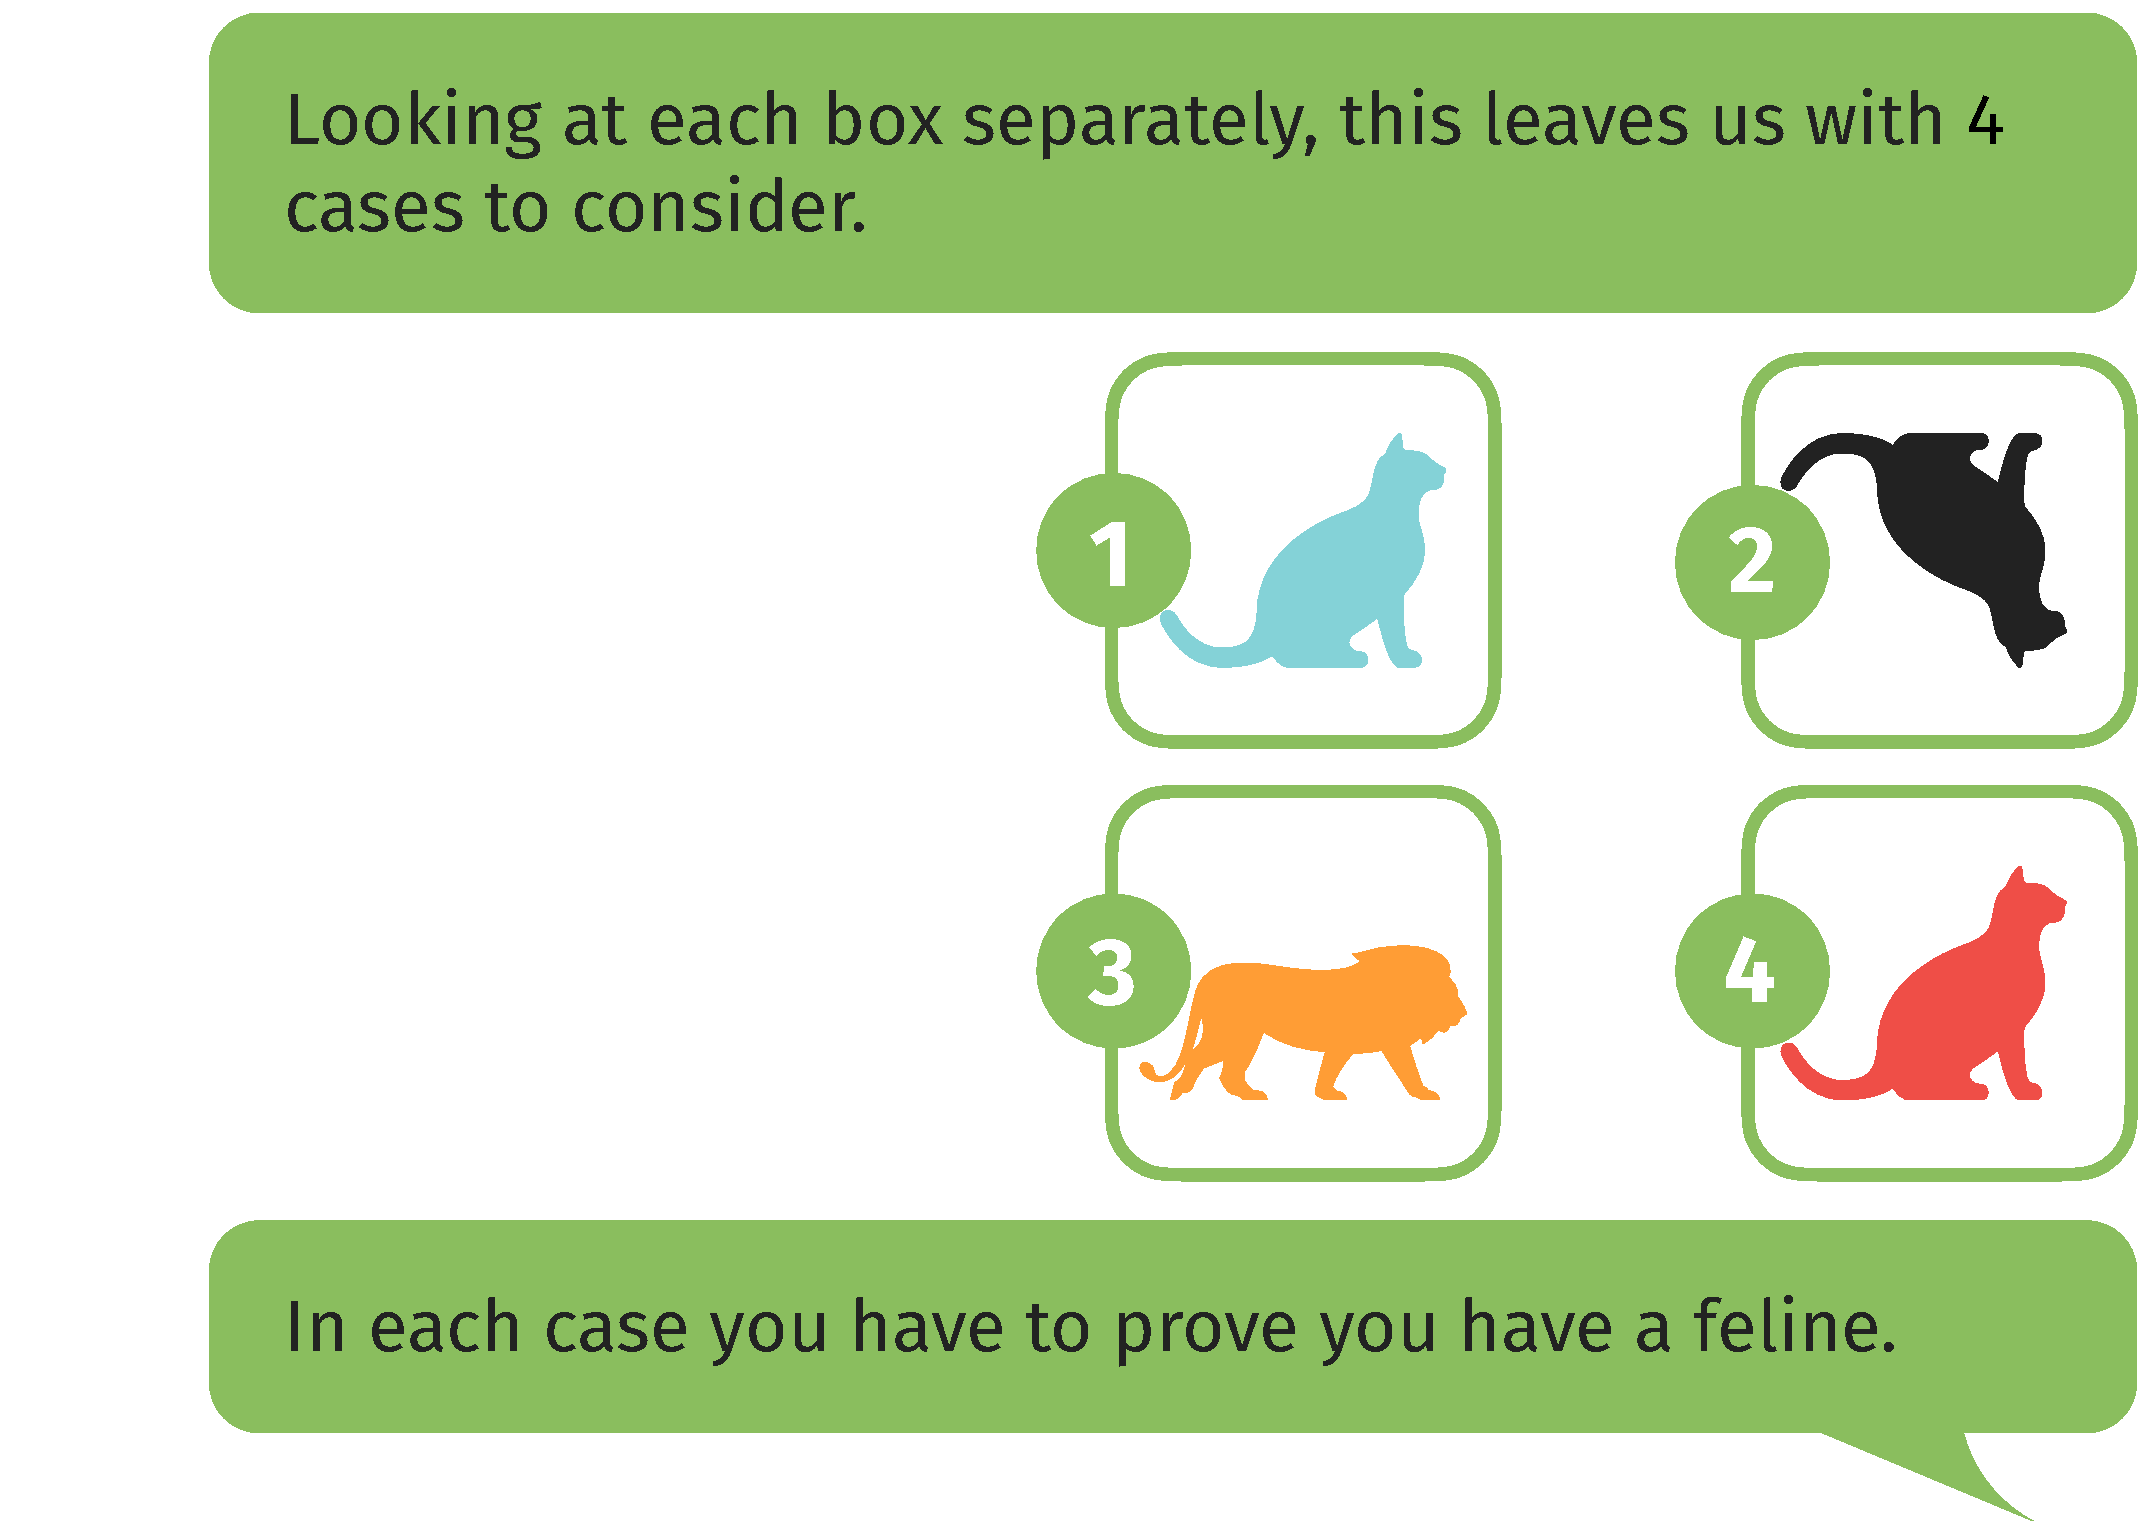
\includegraphics[width=0.8\textwidth]{convo8.pdf}
\end{center}

We are presented with four cases, and as many statements to prove.
In this case, we are rather lazy, especially since all four cases will be
similar. Fortunately for us, the proof assistant is capable of understanding
that you want to deal with several cases in similar ways, \emph{and} is also
capable of doing very basic proofs without the user.

\begin{center}
  
\includegraphics[width=0.8\textwidth]{convo9.pdf}
  
\includegraphics[width=0.8\textwidth]{convo10.pdf}
\end{center}

Once the proof is complete, the proof assistant tells you so and you can move on
to other theorems to prove. I already showed that you have to be explicit and
non ambiguous when talking to the proof assistant. You also have to be correct.
The proof assistant will not trust blindly into what you say.
%
Let us now consider a theorem that is not provable.

\begin{center}
  
\includegraphics[width=0.8\textwidth]{convo11.pdf}
  
\includegraphics[width=0.8\textwidth]{how-to-prove.pdf}
  
\includegraphics[width=0.8\textwidth]{convo7.pdf}
  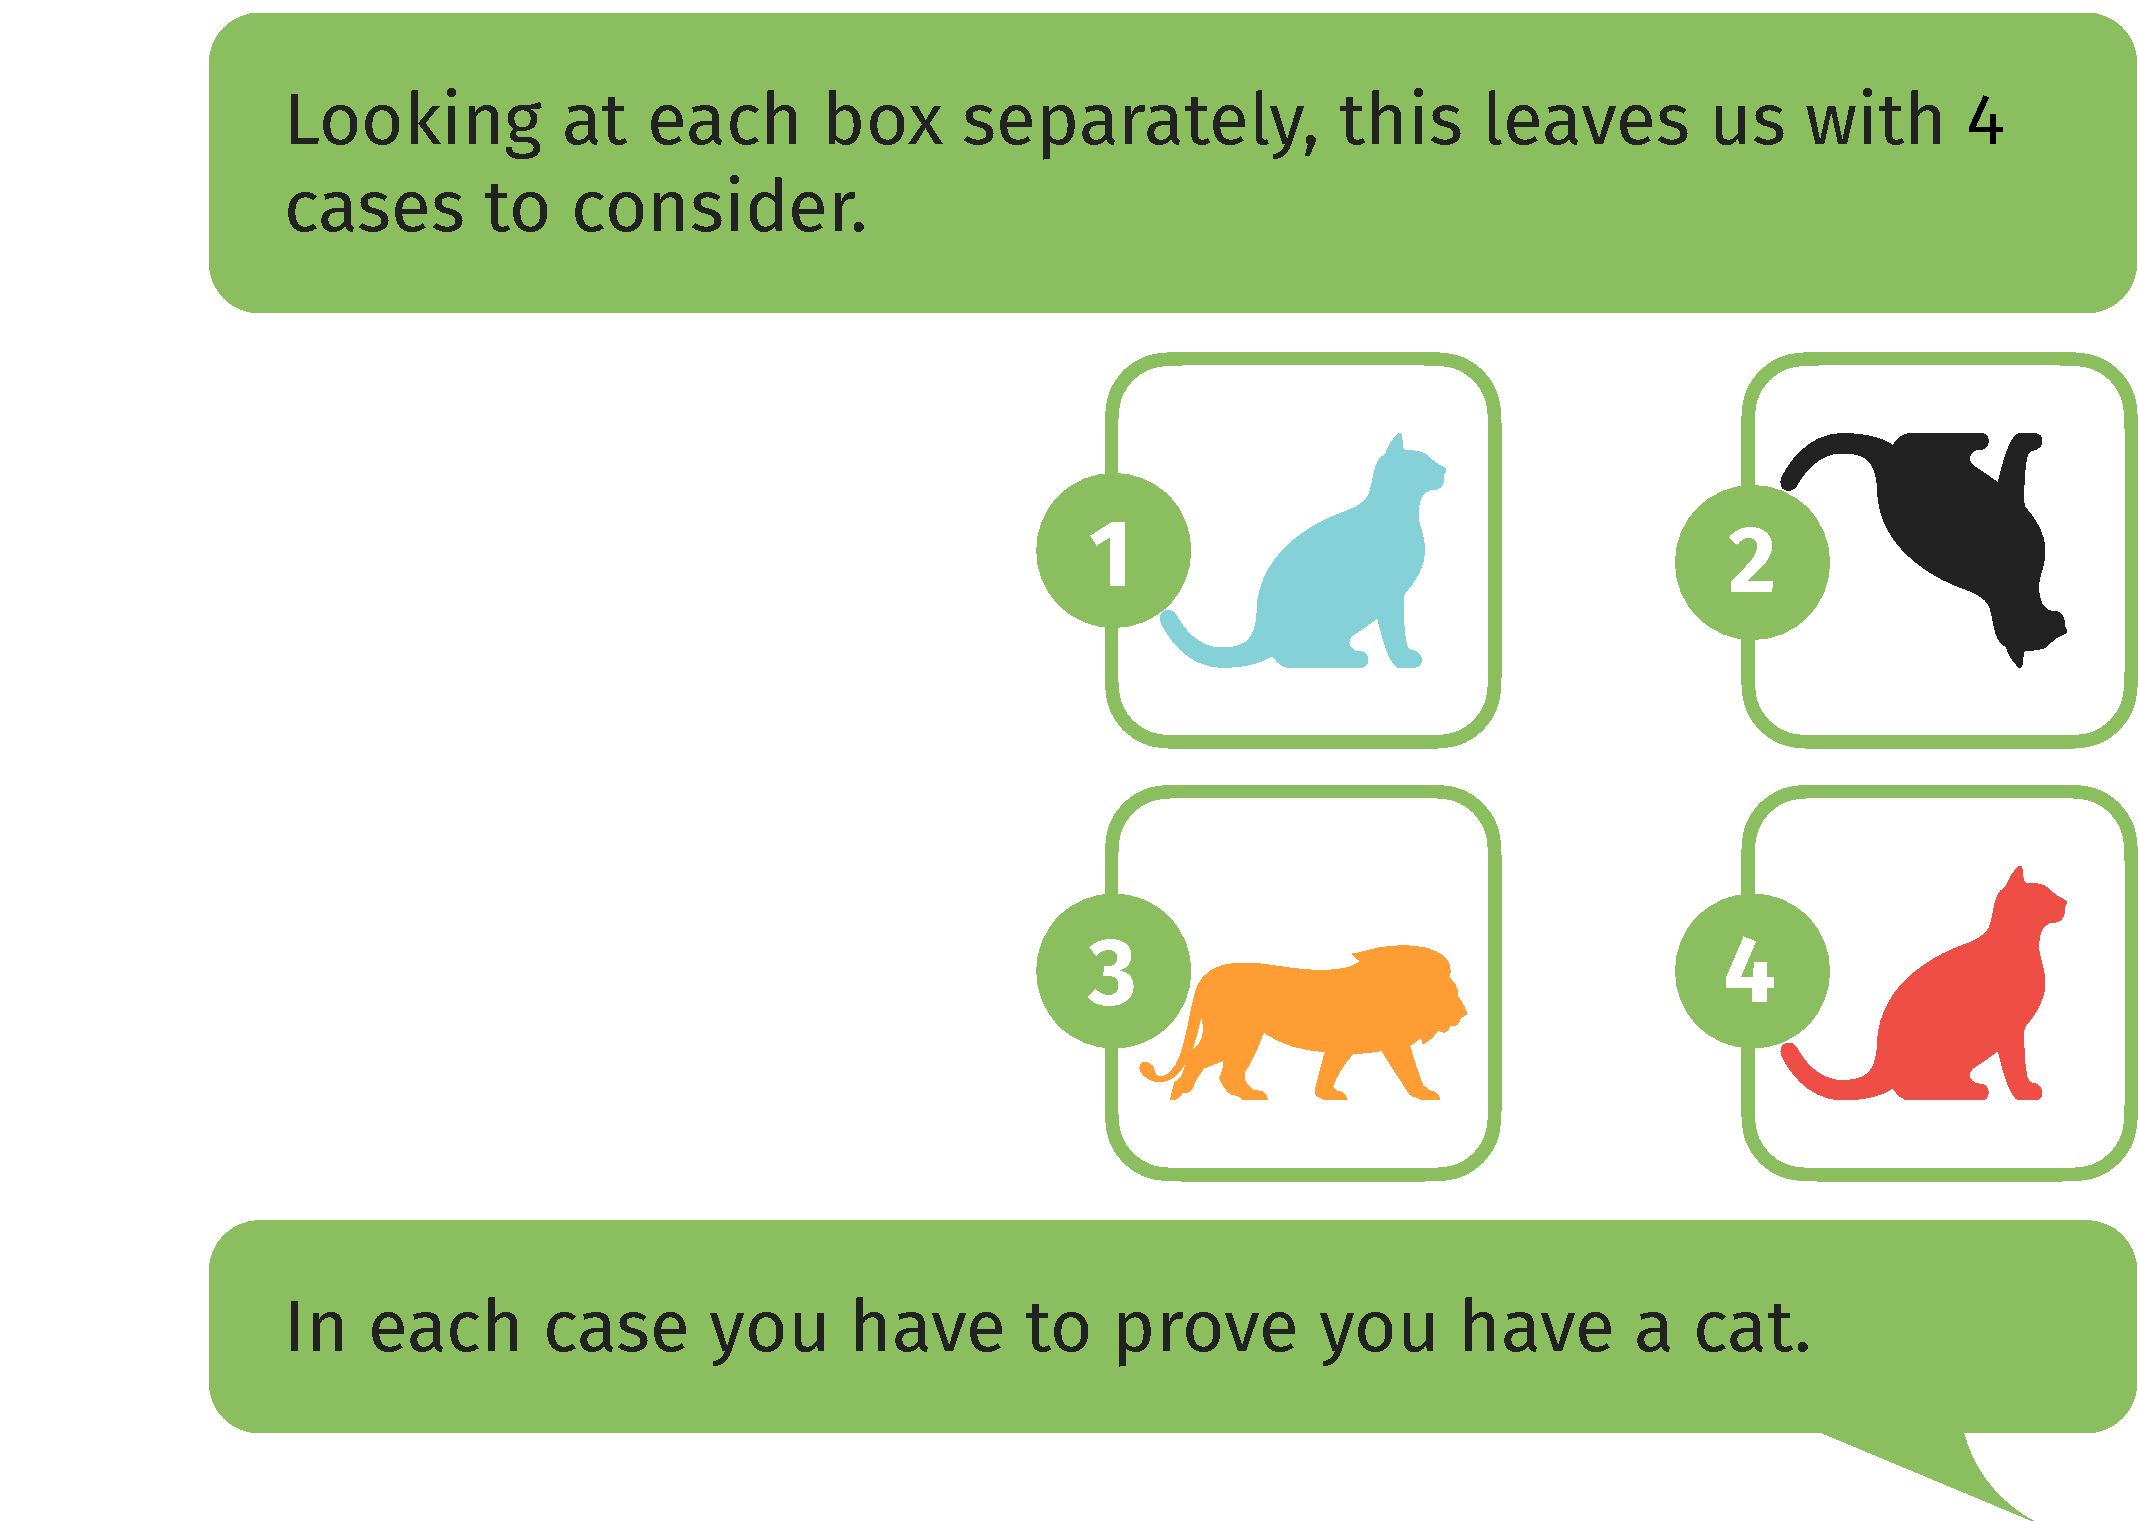
\includegraphics[width=0.8\textwidth]{convo12.pdf}
  
\includegraphics[width=0.8\textwidth]{convo9.pdf}
  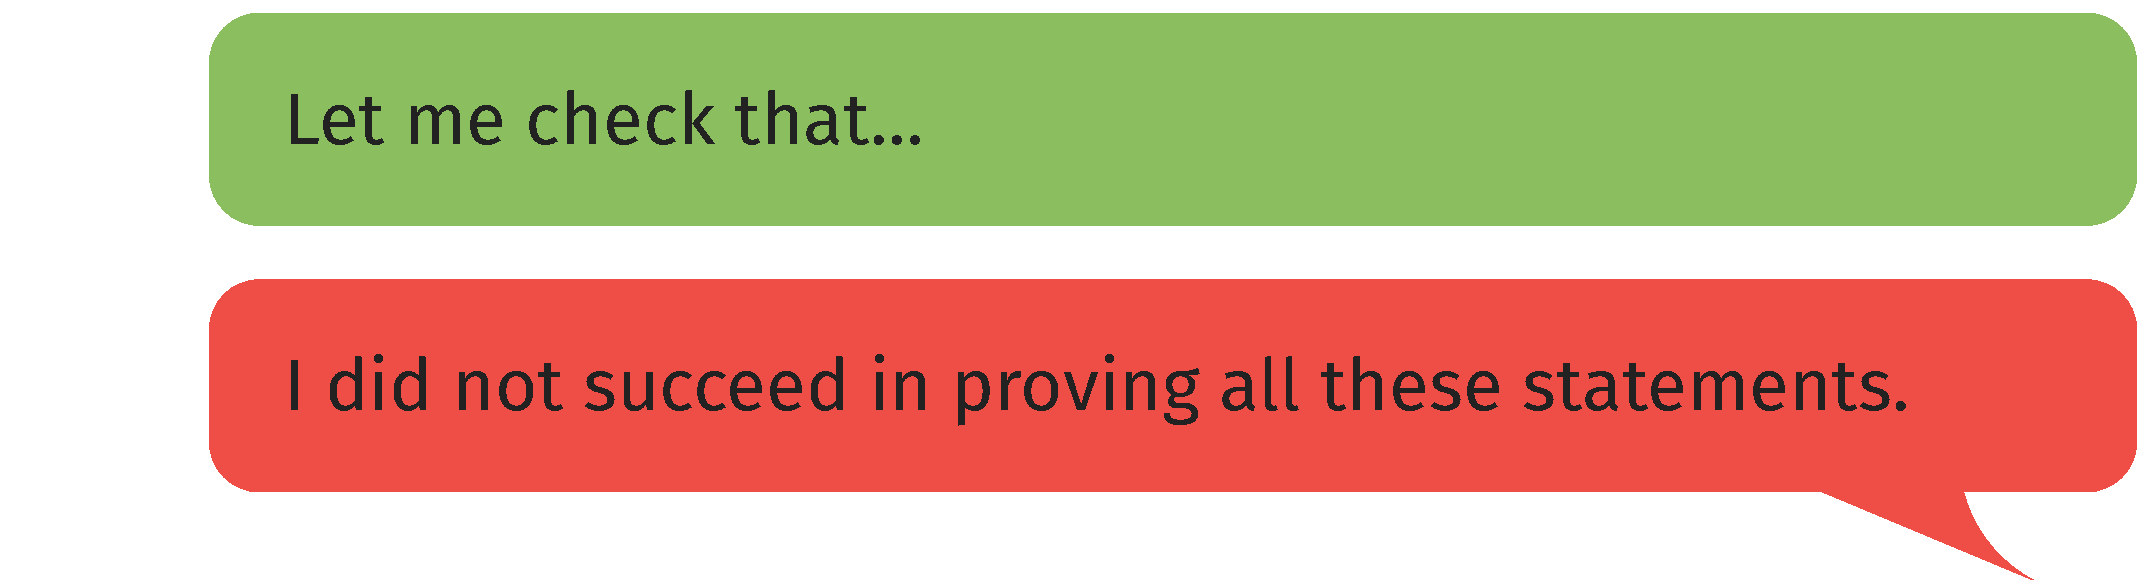
\includegraphics[width=0.8\textwidth]{convo13.pdf}
  
\includegraphics[width=0.8\textwidth]{convo-focus.pdf}
  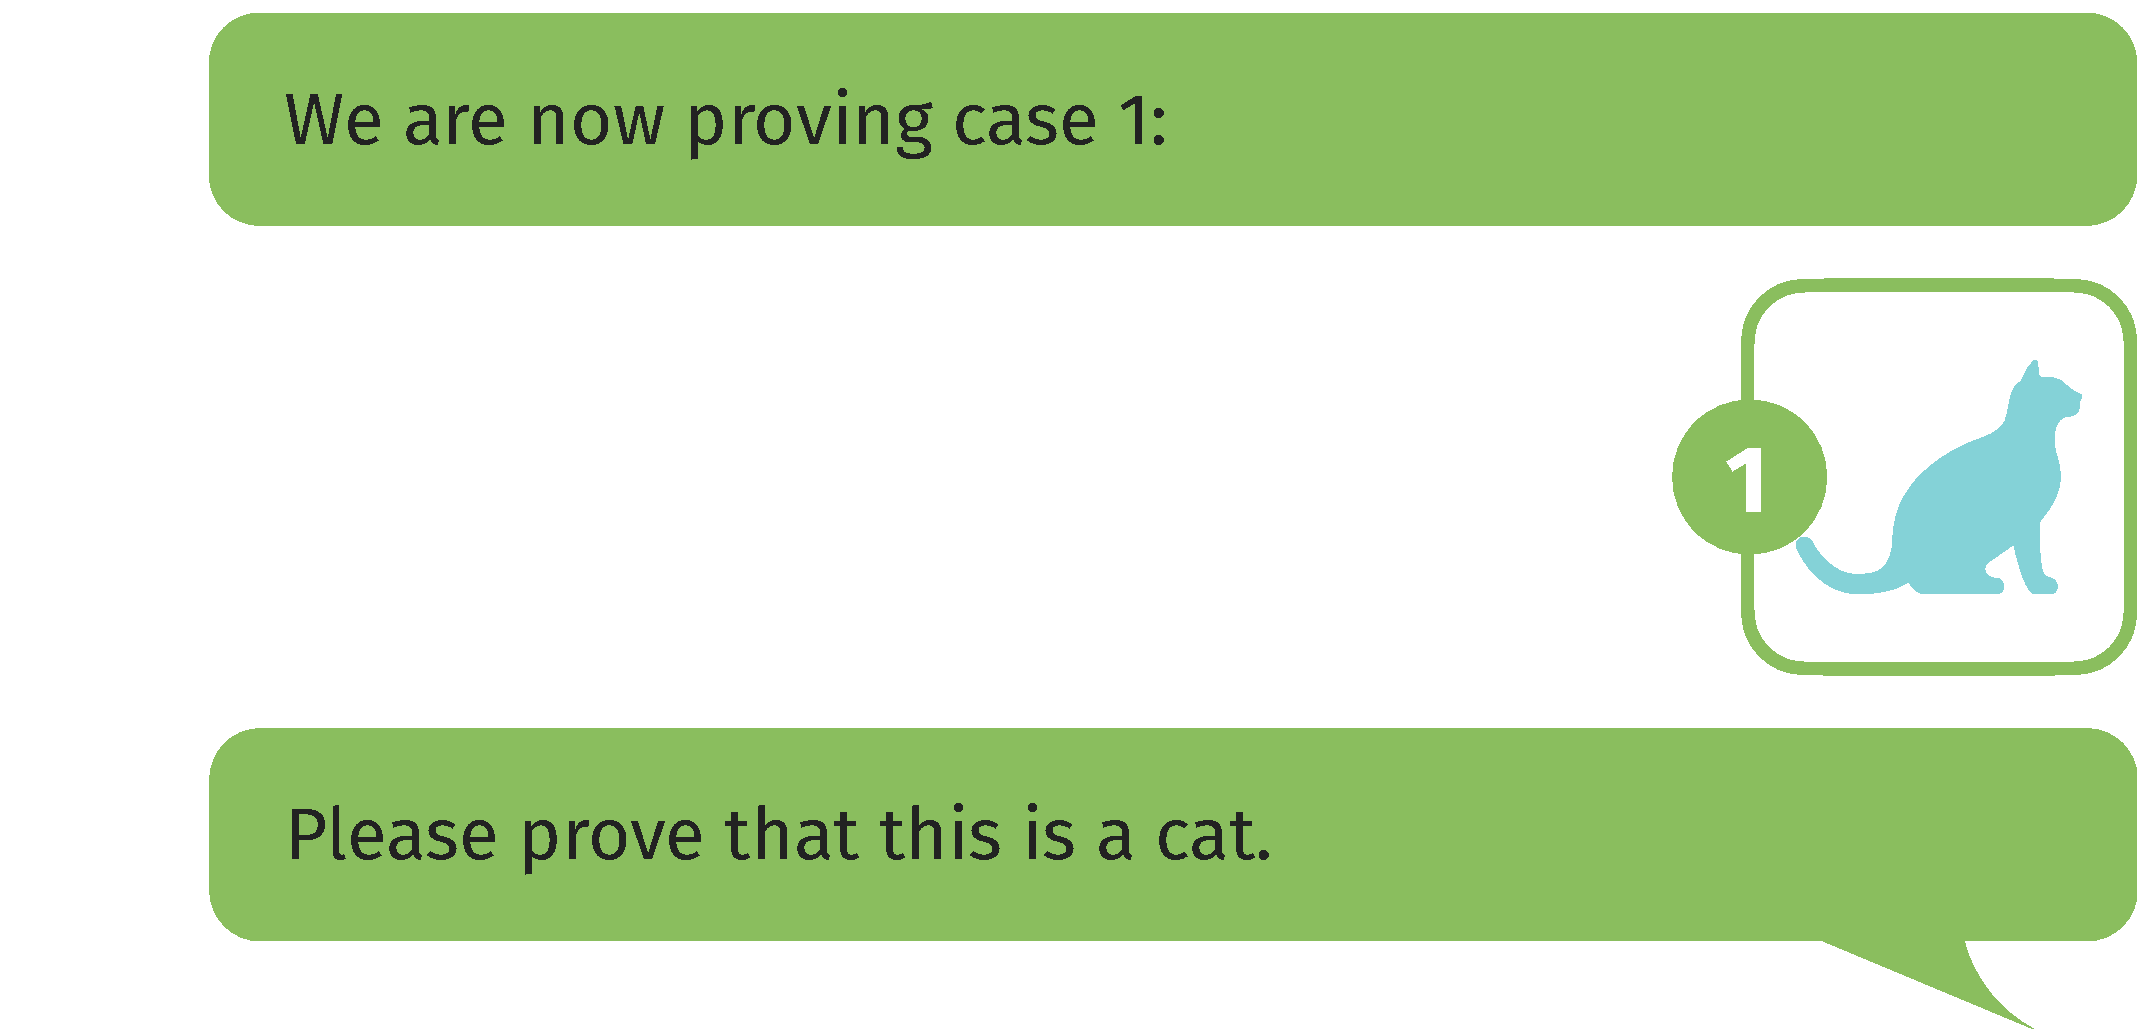
\includegraphics[width=0.8\textwidth]{convo-case1.pdf}
  
\includegraphics[width=0.8\textwidth]{convo-trivial.pdf}
  
\includegraphics[width=0.8\textwidth]{convo-indeed.pdf}
  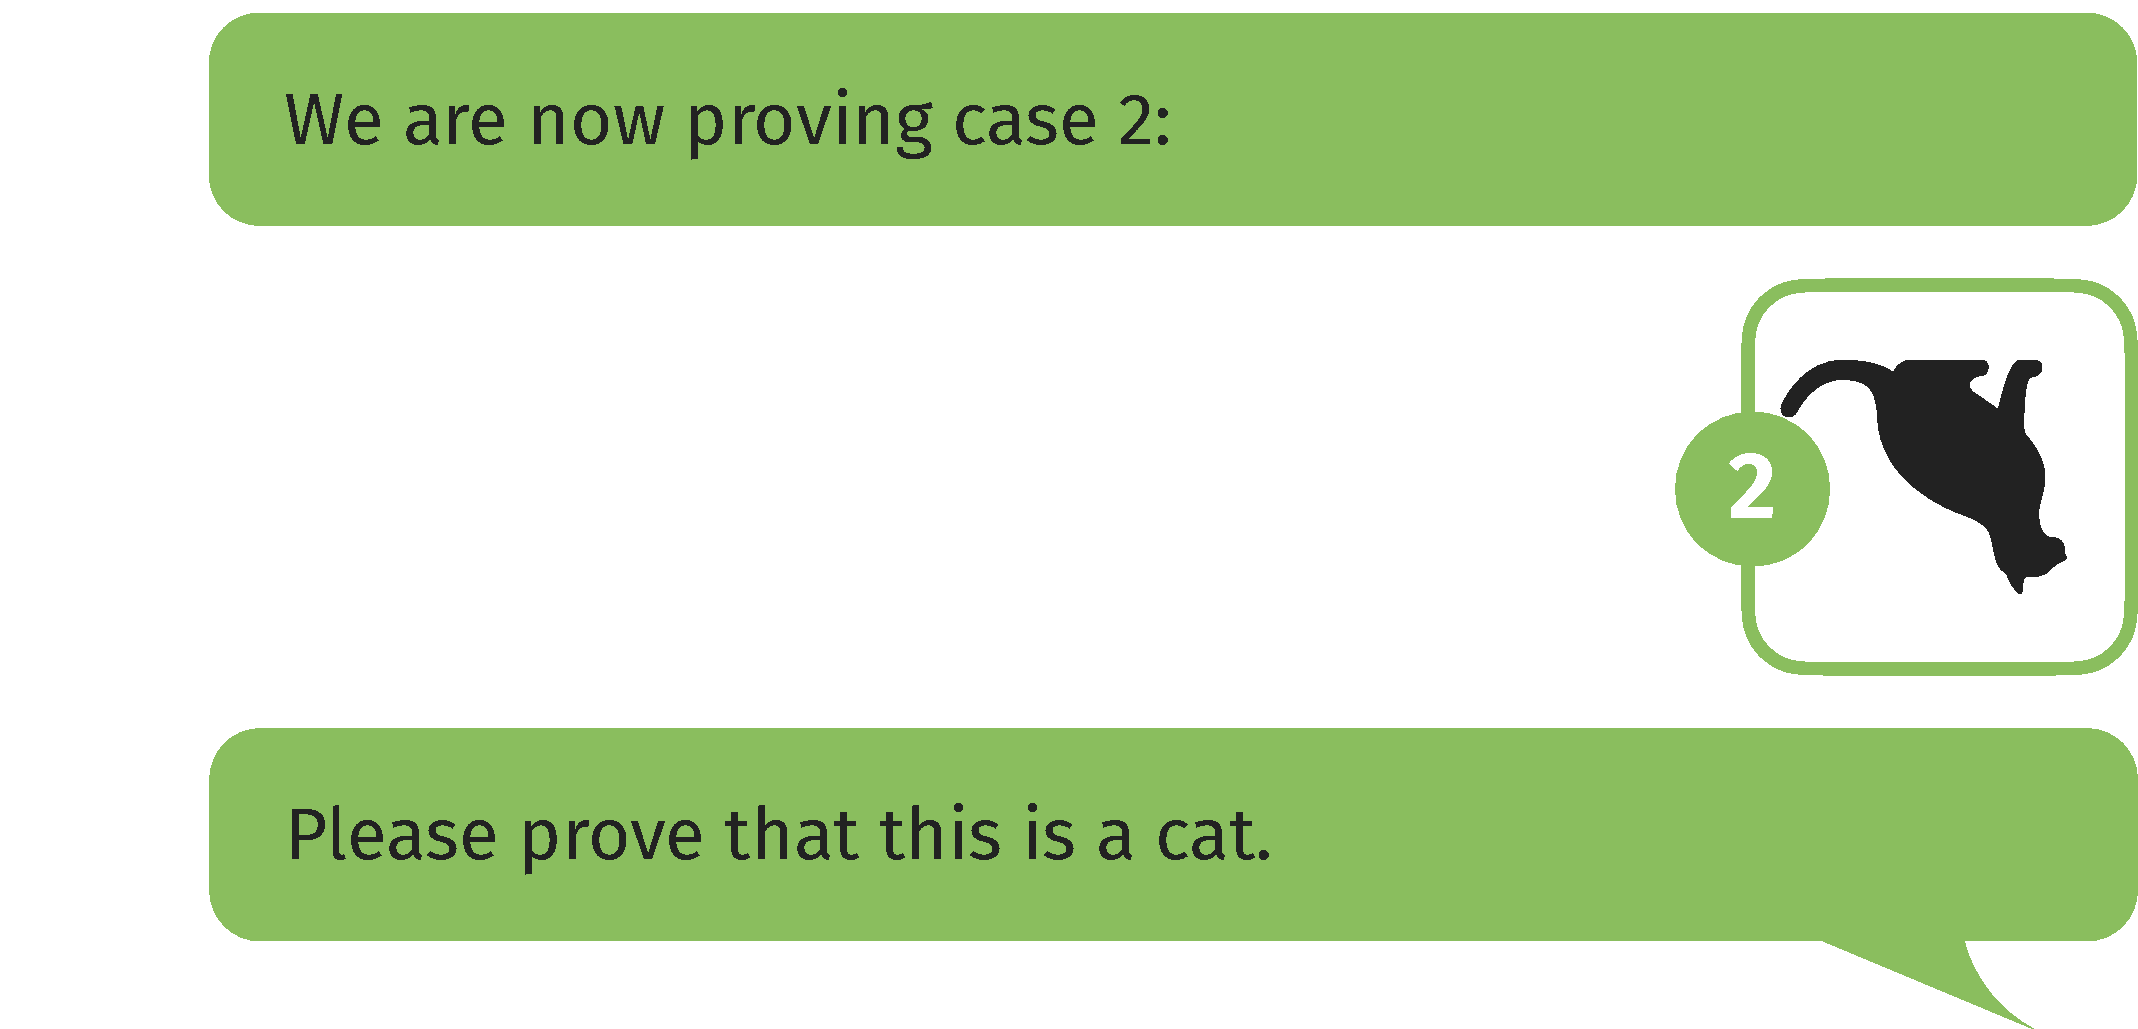
\includegraphics[width=0.8\textwidth]{convo-case2.pdf}
  
\includegraphics[width=0.8\textwidth]{convo-trivial.pdf}
  
\includegraphics[width=0.8\textwidth]{convo-indeed.pdf}
  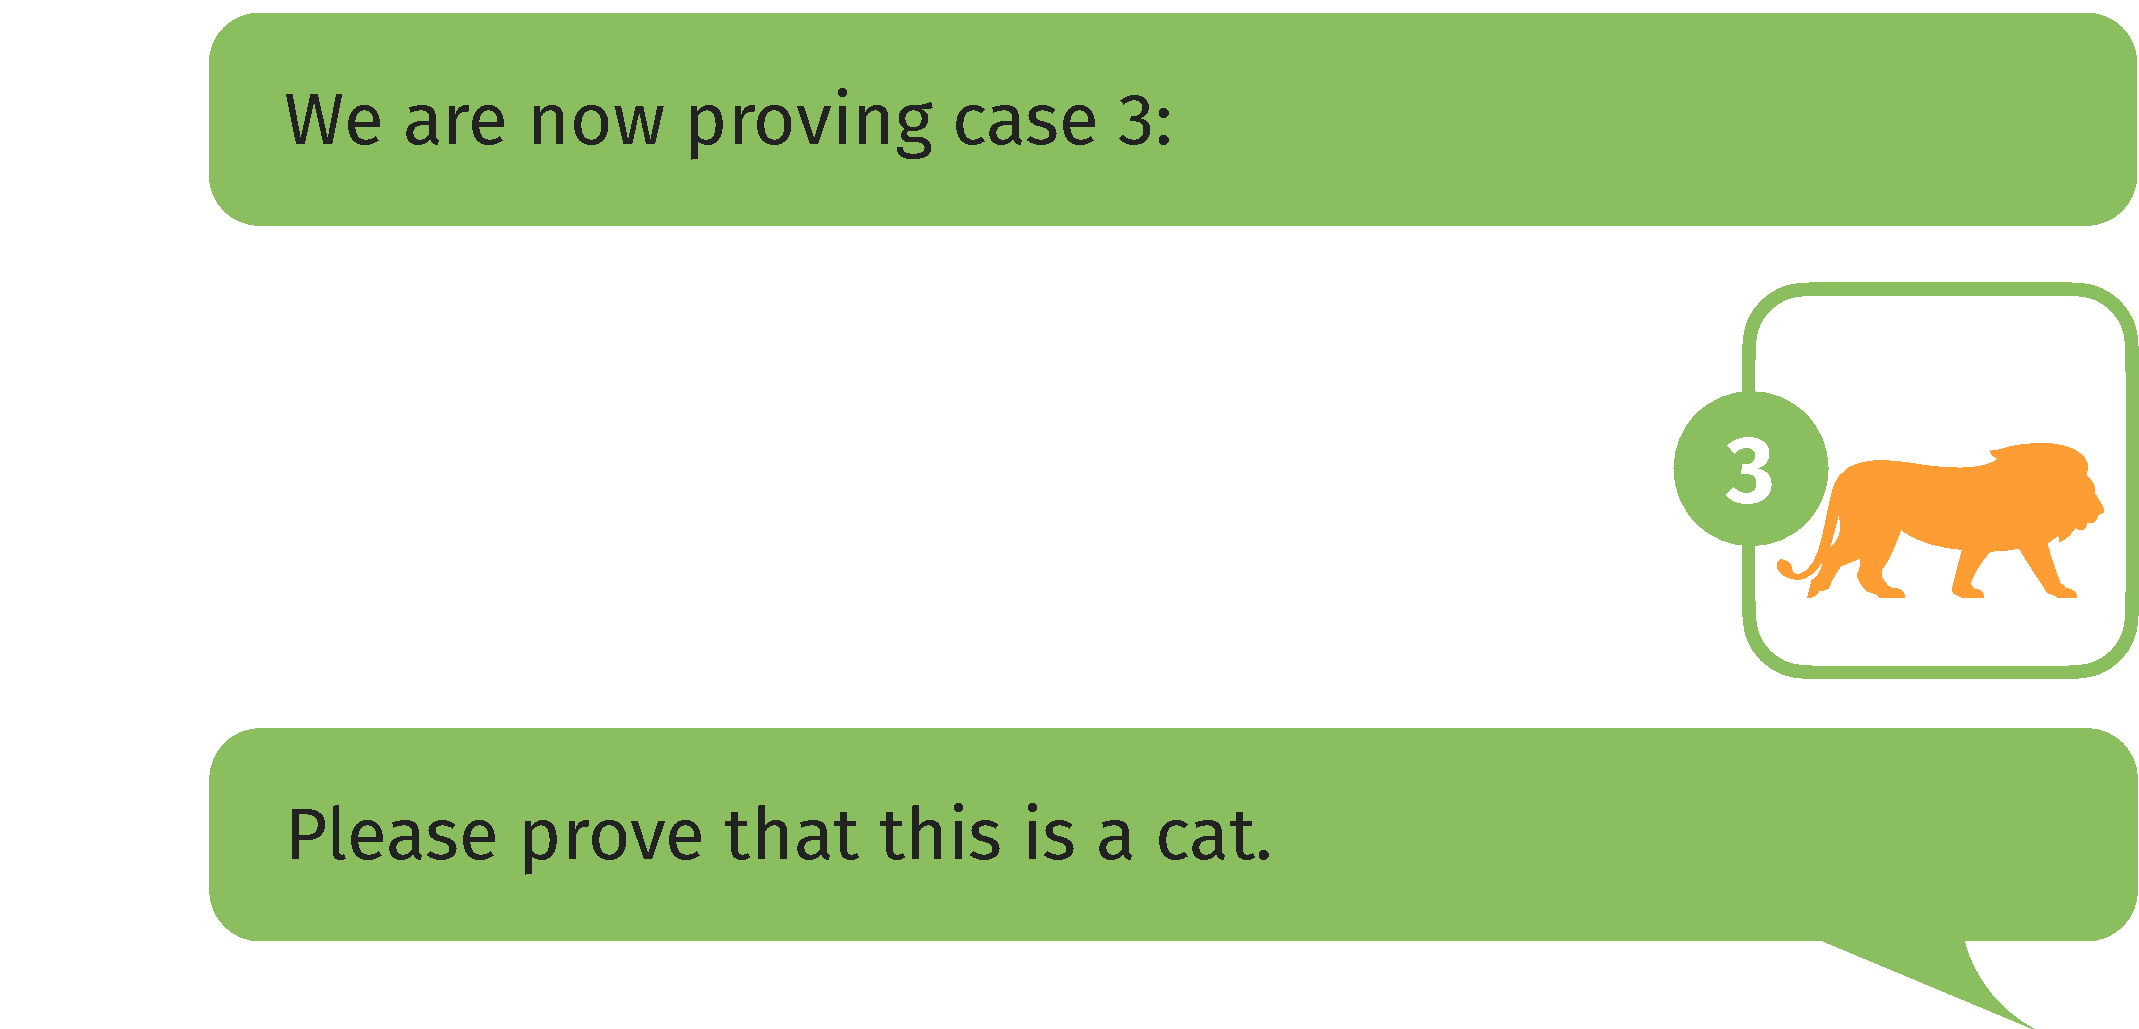
\includegraphics[width=0.8\textwidth]{convo-case3.pdf}
  
\includegraphics[width=0.8\textwidth]{convo-abort.pdf}
\end{center}

It was not a cat...